% Feature importance figure spans both columns — place before \section so LaTeX
% can float it to the top of the methodology page.
\begin{figure*}[t]
    \centering
    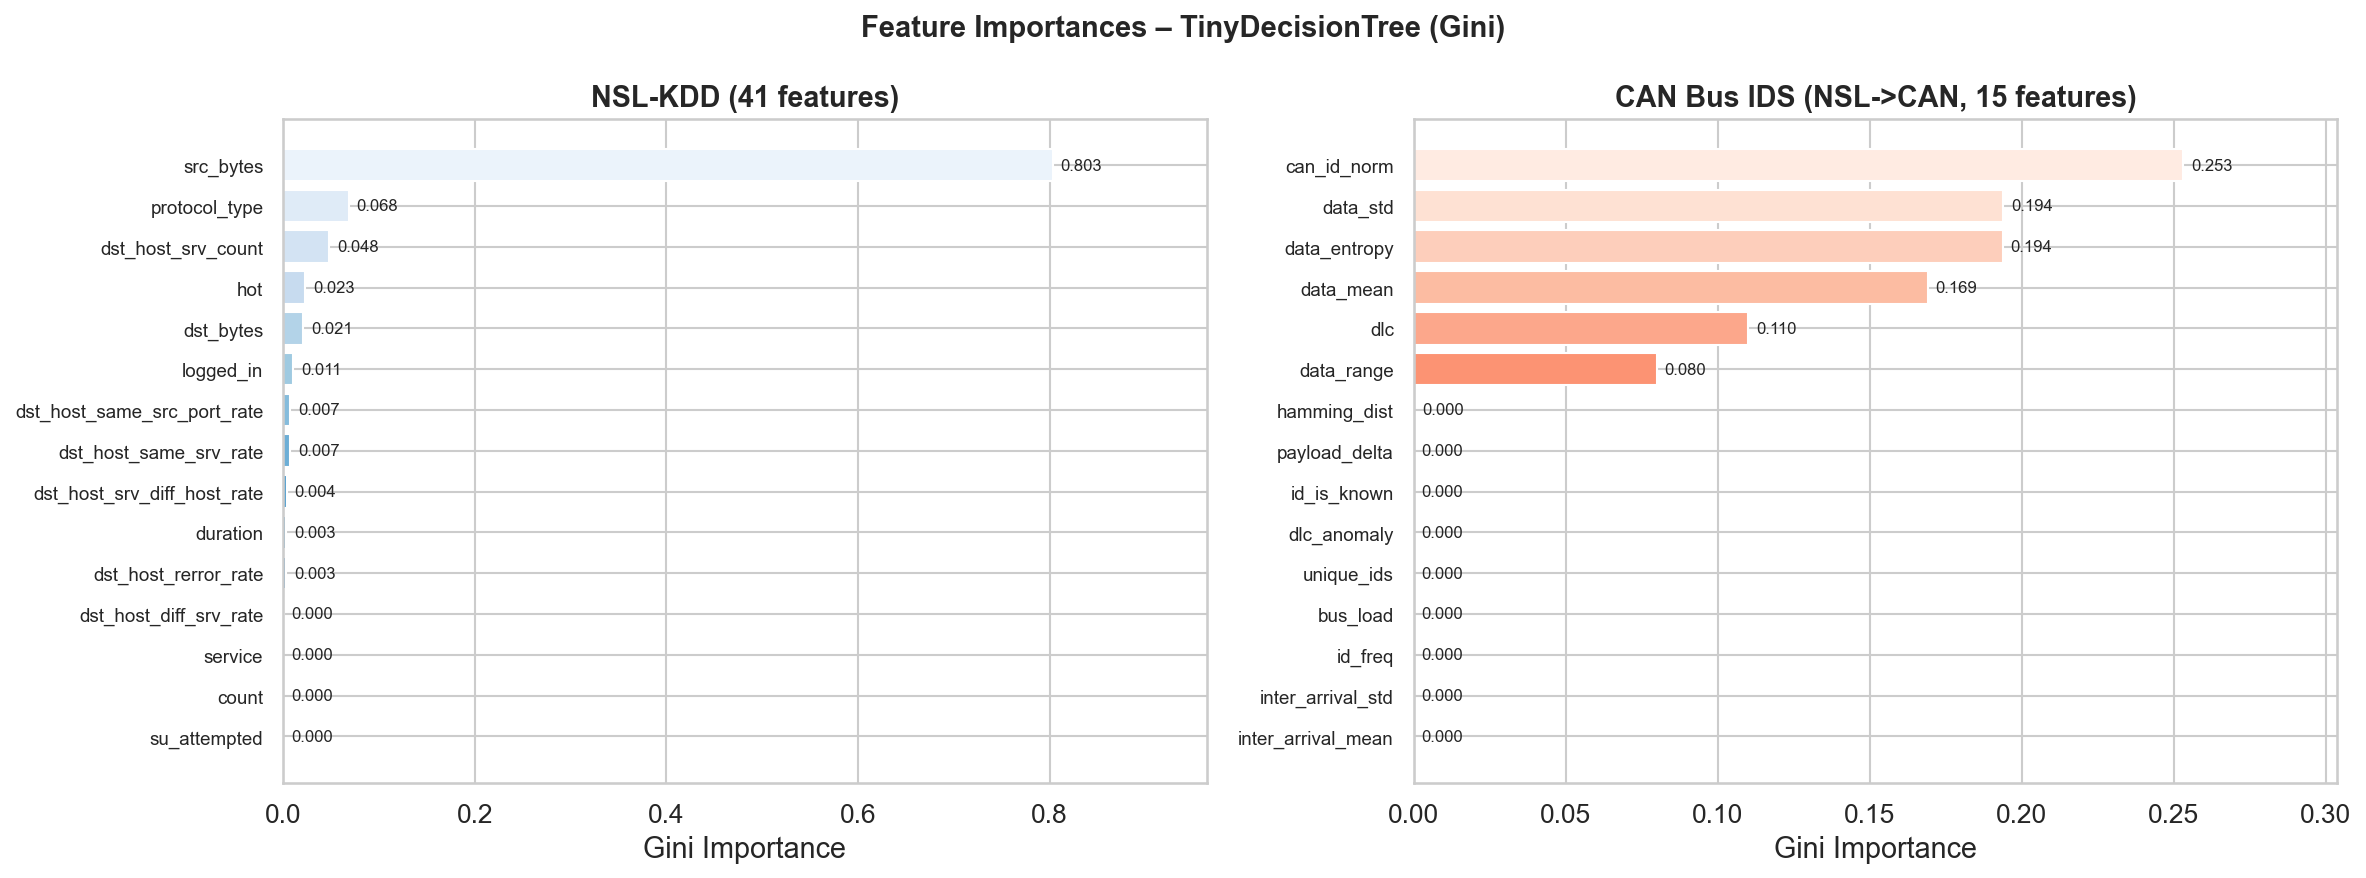
\includegraphics[width=\linewidth]{images/09_feature_importance.png}
    \caption{Gini impurity importances for the deployed TinyDecisionTree on NSL-KDD (left, 41 network features) and the Satellite CAN IDS (right, 15 CAN features).}
    \label{fig:feature_importance}
\end{figure*}

% ------------------------------------------------------------------
\section{Methodology}
\label{sec:methodology}
% ------------------------------------------------------------------

In the following section we describe the five-stage pipeline we have developed from training to inference. All computationally intensive tasks, including dataset generation, feature extraction, model training, threshold analysis, quantization, and C-code export, are conducted offline using ground infrastructure. The microcontroller is responsible solely for executing a bounded, heap-free inference path. To maintain clarity and reproducibility, we organize the paper such that all methodological details, including the design of our five-stage pipeline, candidate model selection, and offline benchmarking, are presented in this section. In Section~\ref{sec:results}, we present the results of the deployed system, focusing on online evaluation, hardware performance, and live experimental outcomes.

\begin{comment}
    
\subsection{End-to-End Pipeline}

The system implements a five-stage pipeline that enforces a strict separation between ground-side training and onboard inference. All computationally intensive tasks, including dataset generation, feature extraction, model training, threshold analysis, quantization, and C-code export, are conducted offline using ground infrastructure. The microcontroller is responsible solely for executing a bounded, heap-free inference path.

\begin{enumerate}
    \item \textbf{CAN traffic generation.} Labeled satellite CAN bus traffic is produced by the SATLL hardware under two controlled experimental regimes (Section~\ref{sec:experiments}), with synthetic attack injections applied at controlled rates.
    \item \textbf{Feature extraction.} A sliding window of 50 frames is maintained as frames arrive; 14 features are computed per frame.
    \item \textbf{Model training and selection.} Five candidate classifiers are benchmarked; the depth-constrained decision tree is selected for its sub-kilobyte flash footprint and sub-microsecond latency.
    \item \textbf{Quantization-aware export.} The trained tree and scaler parameters are exported as static C arrays in three numeric formats (float32, int16, int8) for flash-footprint comparison.
    \item \textbf{Firmware integration.} The C header is linked into a STM32 build. Inference is driven by the host-side runner over USB OTG (CDC ACM) for benchmarking; onboard autonomous monitoring is the operational target.
\end{enumerate}

\end{comment}


% ------------------------------------------------------------------
\subsection{CAN Feature Engineering}
\label{sec:features}
% ------------------------------------------------------------------

A total of fourteen features are extracted from an offline 50-frame sliding window over the raw CAN bus stream. These features are categorized as payload structure, temporal dynamics, and bus topology, as detailed in Table~\ref{tab:features}. The sliding window maintains per-ID history, ensuring that per-ID timing statistics remain computable even in a shared bus environment.

Scaling parameters ($\mu$, $\sigma$) are estimated from the training corpus and stored as 30 float32 constants (120 bytes) alongside the decision tree. During inference, each feature value is z-scored using these constants prior to tree evaluation.

% ------------------------------------------------------------------
\subsection{Candidate Model Evaluation and Selection}
\label{sec:model_selection}
% ------------------------------------------------------------------

Five model architectures are benchmarked on real-world network-IDS datasets (UNSW-NB15 and NSL-KDD \cite{UNSW2015, NSLKDD2009}) to establish the trade-off between resource usage and accuracy prior to domain-specific CAN training. The evaluated candidates include a shallow TinyDecisionTree (depth $\leq$ 5), TinyXGBoost and MicroXGBoost (with 3 and 5 gradient-boosted trees, respectively), a LightRandomForest (10 trees), and a CompactExtraTrees ensemble (8 trees). Each model is assessed based on recall, F1-score, ROC-AUC, serialized flash size, and per-sample inference latency. Comprehensive benchmark results are presented in Table~\ref{tab:model_comparison}. On UNSW-NB15 all models achieve similarly high recall ($\geq$98.9\%), so the differentiating axes are flash footprint and inference latency. The ensemble methods (LightRandomForest at 106~KB, CompactExtraTrees at 41~KB) are immediately eliminated by the CubeSat flash constraint; their 14\,ms per-sample latency would consume an impractical share of the OBDH task budget. MicroXGBoost and TinyXGBoost occupy 6--10~KB and 260--320~\textmu s—below the flash threshold but two orders of magnitude slower than the decision tree. On NSL-KDD, TinyXGBoost achieves slightly higher recall (69.2\% vs 65.7\%) but at the cost of 10$\times$ the inference time.

TinyDecisionTree is the only model meeting all three embedded constraints simultaneously: $<$6~KB serialized size, $<$30~\textmu s inference on host CPU, and recall $\geq$65\% across both datasets. It is selected for all subsequent CAN-domain training and firmware integration.

\begin{table}[t]
\caption{All candidate models on UNSW-NB15 and NSL-KDD real-world benchmarks. \textbf{Bold}: selected for embedded deployment. Latency measured on host CPU.}
\label{tab:model_comparison}
\small
\begin{tabular}{@{}llrrrrr@{}}
\toprule
\textbf{Model} & \textbf{Dataset} & \textbf{Rec.} & \textbf{F1} & \textbf{AUC} & \textbf{Size} & \textbf{Lat.} \\
               &                  & (\%)          & (\%)        &              & (KB)          & (\textmu s)   \\
\midrule
\multirow{2}{*}{\textbf{TinyDecisionTree}}
  & UNSW-NB15 & \textbf{99.4} & \textbf{85.2} & 0.930 & \textbf{5.1}  & \textbf{29} \\
  & NSL-KDD   & \textbf{65.7} & \textbf{78.1} & 0.795 & \textbf{5.2}  & \textbf{29} \\
\midrule
\multirow{2}{*}{TinyXGBoost}
  & UNSW-NB15 & 99.5 & 81.5 & 0.863 & 6.6 & 262 \\
  & NSL-KDD   & 69.2 & 80.0 & 0.896 & 6.6 & 318 \\
\midrule
\multirow{2}{*}{MicroXGBoost}
  & UNSW-NB15 & 99.8 & 83.0 & 0.927 & 9.7 & 259 \\
  & NSL-KDD   & 65.0 & 77.6 & 0.920 & 9.7 & 272 \\
\midrule
\multirow{2}{*}{LightRandomForest}
  & UNSW-NB15 & 99.6 & 85.1 & 0.969 & 106.4 & 14{,}287 \\
  & NSL-KDD   & 65.3 & 78.0 & 0.948 & 118.3 & 14{,}545 \\
\midrule
\multirow{2}{*}{CompactExtraTrees}
  & UNSW-NB15 & 98.9 & 83.2 & 0.880 & 41.3 & 14{,}721 \\
  & NSL-KDD   & 60.1 & 74.6 & 0.886 & 58.7 & 14{,}517 \\
\bottomrule
\end{tabular}
\end{table}

% ------------------------------------------------------------------

% ------------------------------------------------------------------
\subsection{Satellite CAN IDS Training}
\label{sec:can_training}
% ------------------------------------------------------------------

The TinyDecisionTree model is retrained from scratch using the satellite CAN dataset. The training set consists of 25,861 feature vectors derived from labeled satellite CAN frames, while 5,166 held-out frames form the offline test set, with approximately 54.7% attack class representation in each split. The attack class labels include four categories that represent established CAN bus intrusion techniques:

\begin{itemize}
    \item \textbf{DoS}: burst-flooding that saturates the bus
    \item \textbf{Fuzzy}: random-payload injection across all IDs
    \item \textbf{Spoofing}: injection of valid-looking frames under a legitimate ID
    \item \textbf{Replay}: re-transmission of previously captured normal frames
\end{itemize}

The decision tree is limited to a depth of five, resulting in 39 nodes and 20 leaves (Figure~\ref{fig:tree_structure}). Training completes in 57 ms, and the exported C header file is 541 bytes in size. On the offline held-out set, the model achieves 99.86% recall and a 0.9912 ROC-AUC across all four attack classes.

For cross-domain evaluation, the UNSW-NB15 dataset (82,000 test flows, 34 features) and the NSL-KDD dataset (22,000 test samples, 41 features, including 17 previously unseen attack types) are serialized as synthetic CAN streams and processed through the same 14-feature extraction pipeline (Algorithm~\ref{alg:b2can}, Appendix~\ref{app:b2can}). On UNSW-NB15, the offline decision tree achieves 99.43\% recall and a 0.9301 AUC; on NSL-KDD, it achieves 65.73\% recall and a 0.7951 AUC. Figure~\ref{fig:feature_importance} presents the relative feature importances in both domains, Figure~\ref{fig:roc_curves} displays the ROC curves, and Figure~\ref{fig:radar_summary} summarizes the overall model performances.

\begin{figure}[t]
    \centering
    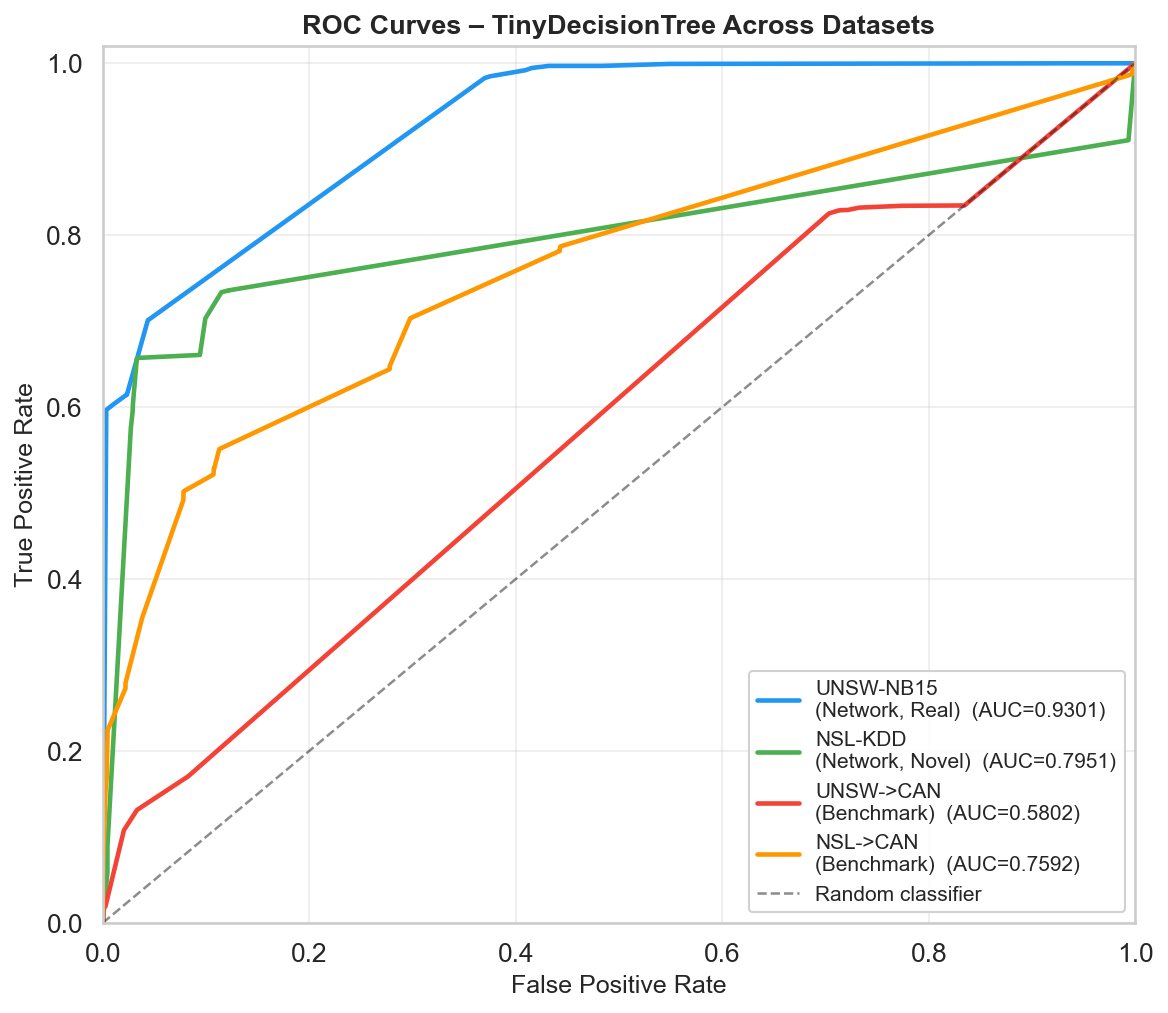
\includegraphics[width=\linewidth]{images/10_roc_curves.png}
    \caption{ROC curves for TinyDecisionTree across deployment domains.}
    \label{fig:roc_curves}
\end{figure}

\begin{figure}
    \centering
    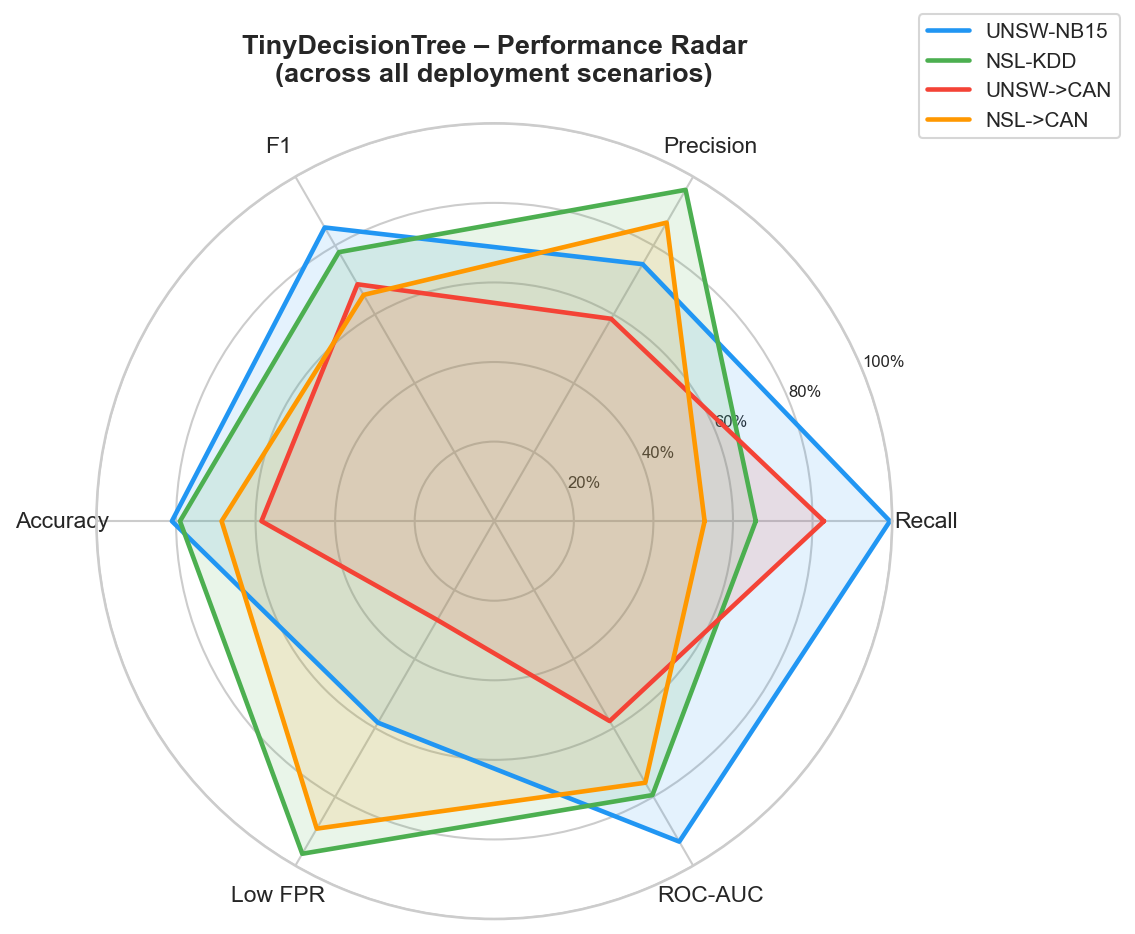
\includegraphics[width=\linewidth]{images/11_radar_summary.png}
    \caption{Radar summary comparing the performance of TinyDecisionTree before and after datasets and benchmarks are converted to CAN format.}
    \label{fig:radar_summary}
\end{figure}

\subsubsection{Benchmark-to-CAN Encoding}

Tabular benchmark samples are serialized as synthetic CAN frame streams. Each stream begins with a meta frame containing the sample index and label, followed by $\lceil F/8 \rceil$ payload frames with min-max-scaled uint8 feature bytes. These streams are then processed through the same 14-feature extraction pipeline as native traffic (Algorithm~\ref{alg:b2can}, Appendix~\ref{app:b2can}). The resulting domain shift quantifies the gap between models trained on network intrusion detection system benchmarks and those deployed in authentic satellite CAN environments.

% ------------------------------------------------------------------
\subsection{Quantization and Model Export}
\label{sec:quantization}
% ------------------------------------------------------------------

Three numeric precision variants of the trained tree are exported as self-contained C headers: Float32 (32-bit IEEE thresholds), Int16 (linearly quantized), and Int8. Float32 is selected for deployment; Int16 is retained as a Cortex-M0/M0+ fallback. Detailed size, latency, and detection-quality comparisons across formats are provided in Appendix~\ref{app:quantization}.


% ------------------------------------------------------------------
\subsection{Firmware Integration and Host-Side Runner}
\label{sec:firmware}
% ------------------------------------------------------------------

For hardware-in-the-loop deployment, the Zubax CANFace CF1 "Babel" served as the CAN-to-host bridge \cite{ZubaxBabelShop2026}. The experimental setup imposed strict constraints on receive buffering, limited to approximately three frames, which required deterministic and lightweight online processing. To meet these requirements, the open-source CANFace CF1 firmware stack \cite{ZubaxCanfaceCF1Repo2026} was modified by replacing the default SLCAN parsing and wrapping path with an inference-oriented acquisition and analysis path specifically designed for IDS benchmarking.

During benchmarking, the STM32 evaluation board is powered by the SATLL payload 5 V rail. A host-side runner streams pre-extracted feature vectors via USB OTG (CDC ACM), while the microcontroller unit (MCU) returns the prediction label, DWT cycle count, and stack high-water mark for each sample. The protocol is detailed in Appendix~\ref{app:protocol}.

Power consumption is measured using SATLL EPS housekeeping telemetry ($P = V_{\text{payload}} \cdot I_{\text{payload}}$), which is logged at 1 Hz. Two quantities are distinguished: the board-level draw, representing the full STM32 evaluation board on the payload rail, and the inference increment, which is the marginal cost of tree traversal alone, bounded by:
\[
    \Delta P_{\text{IDS}} \leq I_{\text{base}} \cdot V_{\text{DD}} \cdot t_{\text{inf}} \cdot f_{\text{poll}},
\]
where $I_{\text{base}}=35$--$38$~mA (measured), $V_{\text{DD}}=3.3$~V, $t_{\text{inf}} \approx 4.2$~\textmu s, and $f_{\text{poll}}=100$~Hz. Complete power measurement results are provided in Section~\ref{sec:res_power}.

% ------------------------------------------------------------------
\subsection{SATLL Experimental Protocol}
\label{sec:experiments}
% ------------------------------------------------------------------

A live evaluation is conducted on the KISPE SATLL using two distinct subsystem experiments. Each experiment comprises two phases: a clean baseline collection phase to characterize normal traffic, followed by an attack injection phase. Attacks are introduced at controlled rates by a separate CAN node connected to the shared bus. The IDS operates continuously during both phases and records labels with microsecond-resolution timestamps.

\subsubsection{Accelerometer Experiment}

The Accelerometer experiment is conducted as part of the Attitude Determination and Control System (ADCS), with a specific focus on the attitude determination component. The objective of this experiment is to demonstrate changes in acceleration across the x, y, and z axes. The satellite's attitude determination capabilities are evaluated by observing varying acceleration values as its position and angle are adjusted. This test is considered effective because it yields relatively stable values for each angle and orientation, resulting in consistent data suitable for research purposes.


\subsubsection{Reaction Wheel Experiment}

The Reaction Wheel experiment is also conducted within the ADCS framework. While it incorporates aspects of attitude determination, its primary emphasis is on the control system. This experiment demonstrates the reaction wheel's operation by spinning the satellite upon activation. As the satellite rotates, corresponding changes in gyro values are observed. The experiment thus evaluates both the satellite’s capability to alter its orientation and to track these changes. Although the data obtained are less consistent than those from the Accelerometer experiment, due to satellite swinging during operation, the test provides a solid foundation and a distinct dataset for further analysis.